%!TEX root = pset1.tex

\section{Linear Basis Function Regression}\label{sec:lin_basis_fn_reg}

\subsection{MLE for Polynomial Basis Function Regression}
We implemented a maximum likelihood estimator for a linear regression with polynomial basis functions, using the formula $\V w = (\M X^T\M X)^{-1} \M X^T\M Y$. The replicated weight vectors are close to what is reported in Table 1.1, and the plots we generated in Figure \ref{fig:bishop_poly_fit} match the ones in Bishop well.

\begin{figure}[h!]
\centering
    \begin{subfigure}[b]{0.4\textwidth}
	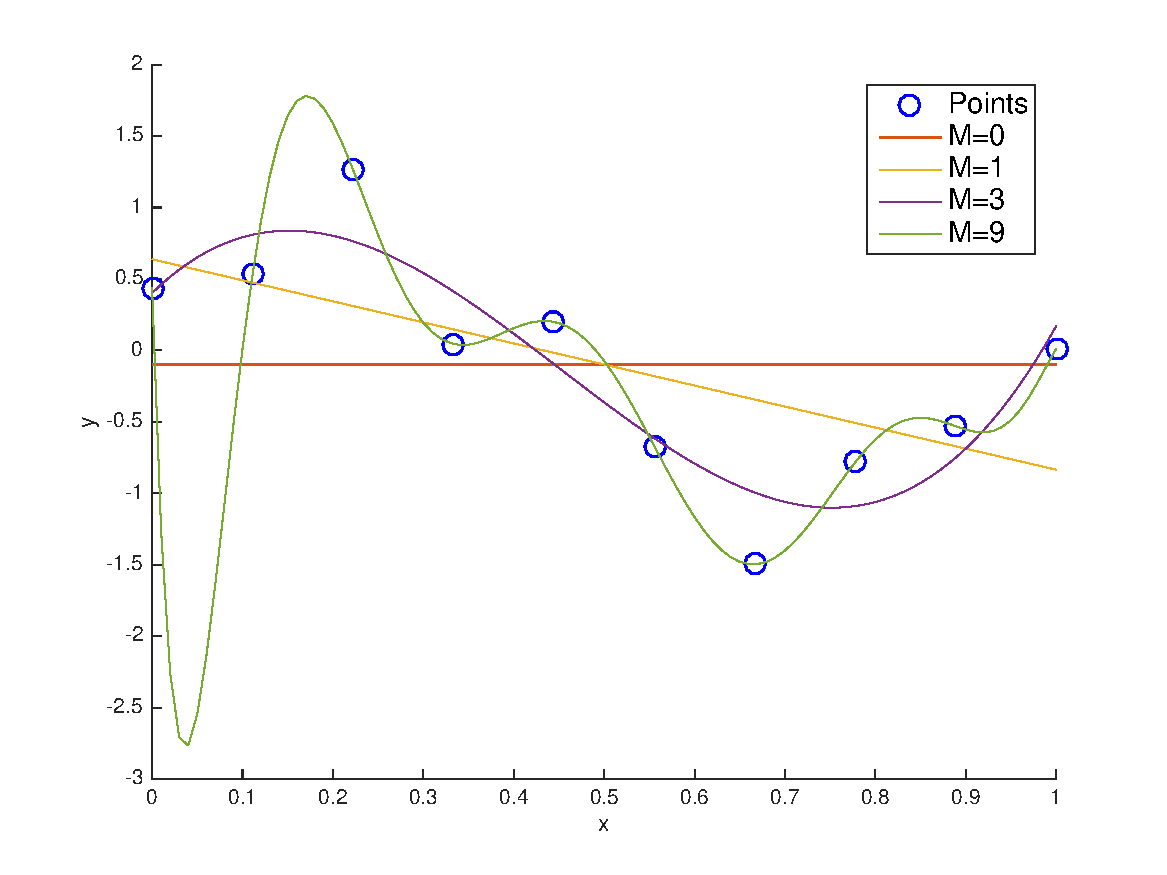
\includegraphics[scale=0.4]{hw1_2.pdf}
	\caption{Replication of Bishop 1.4, using polynomial basis function up to degree $M$.}\label{fig:bishop_poly_fit}
    \end{subfigure}
    \quad
    \begin{subfigure}[b]{0.4\textwidth}
	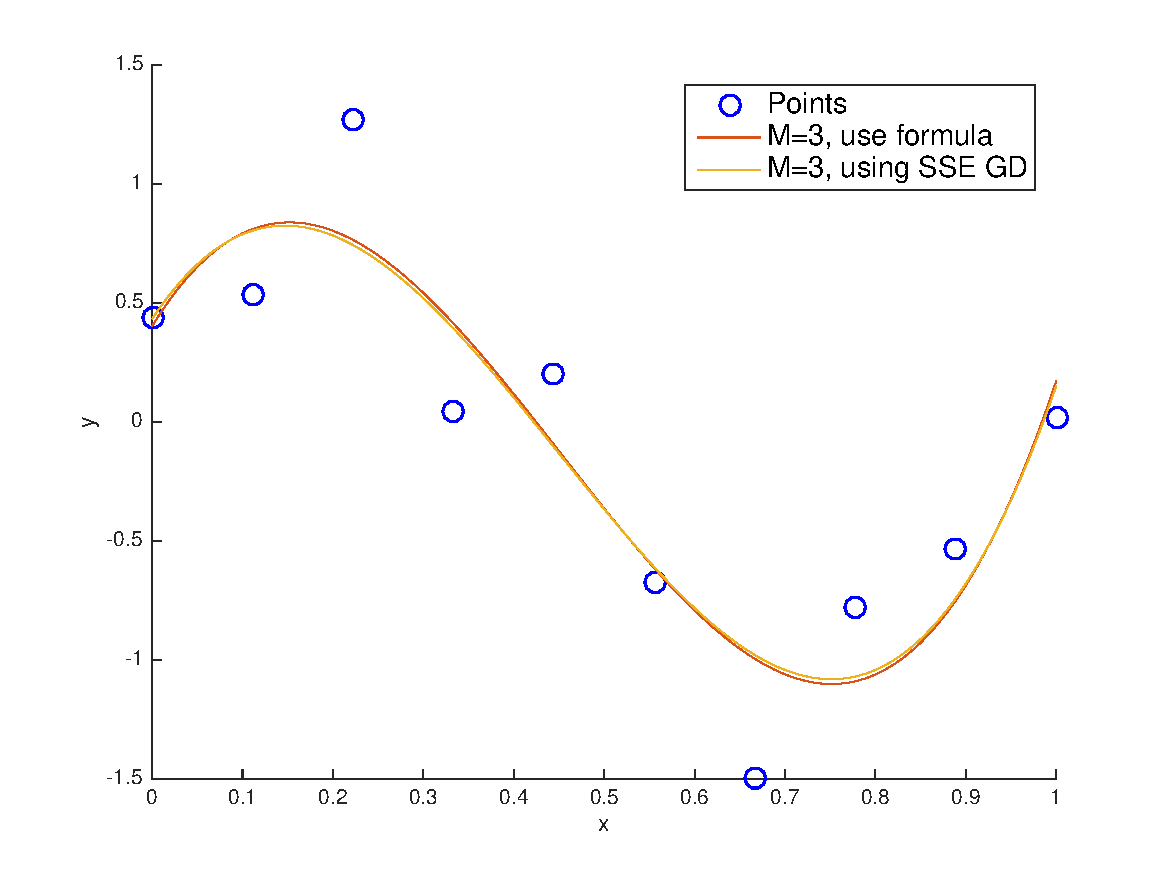
\includegraphics[scale=0.4]{hw1_2_2.pdf}
	\caption{Comparing the estimates using MLE equation or numeric gradient descent on SSE.}\label{fig:bishop_SSE_GD}
    \end{subfigure}
    \quad
    \begin{subfigure}[b]{0.4\textwidth}
	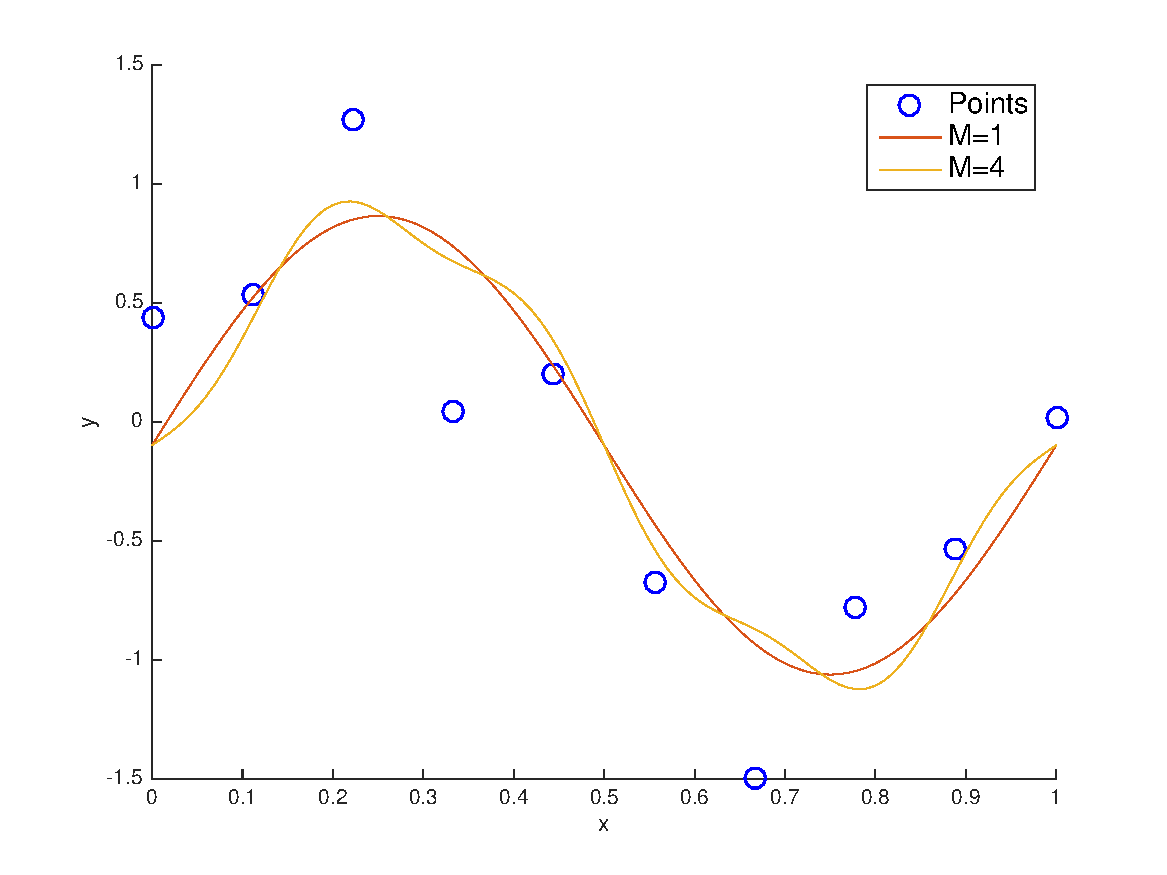
\includegraphics[scale=0.4]{hw1_2_4.pdf}
	\caption{Using sine basis function.}\label{fig:bishop_sin}
    \end{subfigure}  
    \caption{}    
\end{figure}


\subsection{Using SSE}
Alternatively, the maximum likelihood weight vector can be found using numerical gradient descent on the SSE. We first implement code to calculate the SSE: $(\V Y - \V \Phi \V w)^T(\V Y - \V \Phi \V w)$. The derivative is $-2\V \Phi (\V Y - \V \Phi \V w)$, which can also be computed numerically using the finite differencing method implemented in Problem 1. We found that the two methods yield identical gradient values.

\subsection{Use Gradient Descent on SSE to find MLE}
To compute the MLE for $\V w$, we input the SSE as the objective function in the gradient descent method, with $\V w$ as the variable to be optimized over. With a smart initial guess, step size, and reasonably small convergence threshold, our $\V w$ from gradient descent matches the analytic OLS solution closely (within a small margin of error). For example, if the initial guess is within 5\% of the optimum, step size: 0.05, and convergence threshold: $10^{-6}$, then we attain solutions within 1\% of the true weight vector $\V w$.  The comparison can be found in Figure \ref{fig:bishop_SSE_GD}. Some bad choice of step size results in non-convergence or extremely large estimates.   We also compare the speed of the method against the native MATLAB function \texttt{fminunc}.  Given the same convergence criterion, it takes 42 iterations for our method to converge, while \texttt{fminunc} converges after 29 iterations.  


\subsection{Sine Basis Function}
We can also use sine basis functions, with $\phi_1(x) = \sin(2\pi x), \ldots, \phi_M(x) = \sin(2\pi Mx)$. The estimated plots are in Figure \ref{fig:bishop_sin}. We observe that the predicted functions are periodic as expected. One potential disadvantage is that when the underlying data is aperiodic, this estimation cannot capture the trend of non-periodic behavior.  This drawback may be worse for regression problems with out-of-sample data that lies outside the range of observed features, because periodic functions have finite range.

